\documentclass[11pt]{article}
\usepackage[utf8]{inputenc}
\usepackage[english]{babel}
\usepackage{amsmath}
\usepackage{graphicx}
\usepackage{float}
\usepackage{lipsum}
\usepackage{multicol}
\usepackage{xcolor}
\usepackage{tabularx}
\usepackage{booktabs}
\usepackage{hyperref}
\newcolumntype{Y}{>{\centering\arraybackslash}X}
\usepackage[left=2.00cm, right=2.00cm, top=2.00cm, bottom=2.00cm]{geometry}

\title{AN2DL Reports Template}

\begin{document}
    
    \begin{figure}[H]
        \raggedright
        
\includegraphics[scale=0.4]{images/polimi.png} \hfill 
\includegraphics[scale=0.3]{images/airlab.jpeg}
    \end{figure}
    
    \vspace{5mm}
    
    \begin{center}
        % Select between First and Second
        {\Large \textbf{ANNDL - First Homework Report}}\\
        \vspace{2mm}
        % Change with your Team Name
        {\Large \textbf{Neural Network November}}\\
        \vspace{2mm}
        % Team Members Information
        {\large Bettiati Matteo,}
        {\large Bianchi Lorenzo,}
        {\large Ostidich Francesco}\\
        \vspace{2mm}
        % Codabench Nicknames
        {betti,}
        {lolly,}
        {kello}\\
        \vspace{2mm}
        % Matriculation Numbers
        {258730,}
        {259946,}
        {259863}\\
        \vspace{5mm}
        \today
    \end{center}   
    \vspace{5mm}
    
    \begin{multicols}{2}

        \section{Introduction}
        
        This project\cite{lecun2015deep}\cite{polimi_2024_2025} focuses on developing a neural network for multi-class classification of images representing eight distinct blood cell states. The main challenges included addressing class imbalance, generalizing from a relatively small dataset, and ensuring accurate classification. To tackle these, we conducted extensive exploratory data analysis (EDA) to identify and resolve outliers, ambiguities, and class imbalances. A multi-stage data augmentation pipeline, culminating in dynamic augmentation during training, was employed to enhance model generalization.

        We adopted transfer learning, leveraging pre-trained architectures to accelerate learning and adapt the models to the dataset's specific features. Model optimization involved hyperparameter tuning, selective layer unfreezing, and mixed precision training. Our final submission achieved a local accuracy of 96\% and an online evaluation accuracy of 92\%.
        
        \section{Dataset Processing}
        The raw dataset consists of total of 13759 images designed for the classification of different types of blood cells. Each image is labeled with one of eight classes, representing various blood cell types: Basophil, Eosinophil, Erythroblast, Immature granulocytes, Lymphocyte, Monocyte, Neutrophil and Platelet.
        Images size is 96x96, color space is RGB (3 channels), with \textit{uint8} data type.
        
        \subsection{Exploratory Data Analysis (EDA)}

        The first step in the pipeline was performing exploratory data analysis (EDA). We began by plotting a grid sorted by class, which helped us identify two outliers: one image with a Shrek watermark appearing in multiple classes, and another with a Rickroll watermark in the Monocyte class. Both were easily removed as repeated, identical images.
        
        An analysis of class distribution revealed a mild class imbalance, which we addressed through image duplication and data augmentation to ensure more balanced class representation.
        
        We also identified some ambiguously labeled images. Since no images were clearly mislabeled and considering the dataset's size, we chose to retain these ambiguous samples to preserve the dataset's diversity, which can help improve model robustness.
        
        \begin{figure}[H]
            \centering
            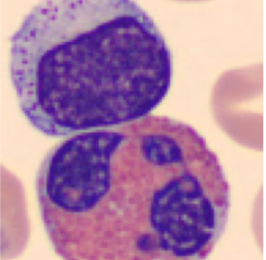
\includegraphics[width=0.15\textwidth]{images/ambiguous1.png}
            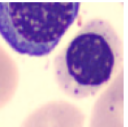
\includegraphics[width=0.15\textwidth]{images/ambiguous2.png}
            \caption{\small Ambiguous samples n°1 and n°2}
        \end{figure}
        
        \subsection{Data Augmentation}
        
        To address class imbalance, we initially used the \textit{class\_weights} argument in \textit{model.fit()} to balance class contributions. However, after balancing the dataset through sample duplication and augmentation, class weighting became unnecessary.
        
        Data augmentation played a crucial role in improving model performance. The pipeline was refined in three stages:
        
        1. \textbf{Initial Augmentation}: Basic transformations (flip, rotation, brightness, contrast, hue, etc.) were applied, expanding the dataset to 2,500 images per class.
        
        2. \textbf{Refined Augmentation}: The second round introduced additional functions (grid mask, color degeneration, cutout, shear), Models were retrained on a larger dataset (5,000 images per class, including the augmented test set).
        
        3. \textbf{Dynamic Augmentation}: The final method used real-time augmentation during training with \textit{TensorFlow Dataset} and \textit{keras\_cv}\cite{keras2015} layers like Augmix\cite{hendrycks2019augmix}, RandomZoom, AutoContrast and RandAugment\cite{cubuk2019randaugment}. wrapped in RandomAugmentationPipeline of \textit{keras\_cv} This approach improved generalization but increased training time.
        

        
        
        \section{Model experiments}
        
        Each team member began by selecting a pre-trained model, and while tweaking hyperparameters and top layers structure, we started to look for the best resulting ones to use.
        
        We started with relatively small models, like \textit{MobileNetV2}, a model known for its favorable trade-off between parameter count and accuracy, as the foundation for our experiments, to leverage fast training and less overfitting risk given the small dataset.
        
        Following this initial setup, we proceeded to design the top layers architecture. 
        Overall, while the specific structures varied slightly between attempts, the core design remained consistent.
        
        \begin{table}[H]
            \centering
            \setlength{\tabcolsep}{5pt}
            \small
            \begin{tabular}{|c|}
                \hline
                \textbf{Layer type} \\ \hline
                Input layer \\ \hline
                Pre-trained base model \\ \hline
                Global average pooling 2D \\ \hline
                Normalization (Group or Batch) \\ \hline
                Dropout (0.2 to 0.4) \\ \hline
                Dense (128 to 1024 neurons, ReLU or GeLU) \\ \hline
                Normalization (Group or Batch) \\ \hline
                Dropout (0.2 to 0.4) \\ \hline
                Dense (64 to 512, ReLU or GeLU) \\ \hline
                Normalization (Group or Batch) \\ \hline
                Dropout (0.2 to 0.4) \\ \hline
                Output layer \\ \hline
            \end{tabular}
        \end{table}
        
        For each dense layer we experimented also with kernel regularizers, with an average value of 1e-3.
        
        By the end we tried a wide range for all parameters as choices like dataset size, complexity, model size and optimizers varied a lot through the experiments.
        Here after a recap with the most used ones.
        
        \begin{table}[H]
            \centering
            \setlength{\tabcolsep}{5pt}
            \small
            \begin{tabular}{|c|c|c|}
                \hline
                \textbf{Parameter} & \textbf{Toptraining} & \textbf{Fine tuning} \\ \hline
                Learning rate & 1e-3 to 1e-4 & 1e-5 to 1e-6 \\ \hline
                Weight decay & 1e-1 to 1e-3 & 1e-1 to 1e-3 \\ \hline
                Epochs & 10 to 20 & 20 to 30 \\ \hline
                Batch size & 32 to 512 & 32 to 512 \\ \hline
            \end{tabular}
        \end{table}
        
        We experimented with two optimizers, \textit{Lion} and \textit{AdamW}, tuning their hyperparameters for optimal performance. \textit{Lion} performed best with a low learning rate and high weight decay, while \textit{AdamW} favored a higher learning rate and lower weight decay.

        Extensive training test runs were conducted to identify the best model parameters based on local test set accuracy. Although the final model used alternative parameters, the hyperparameter tuning provided valuable guidance, with detailed results available in the "\textit{misc/hyperparameter\_tuning.pdf}" file.

        \subsection{Transfer Learning}
        
        The transfer learning process was structured into two phases: training the top layers followed by fine-tuning. The first phase primarily focused on tuning the top layers' architecture and parameters. To enhance training efficiency, we incorporated callbacks such as early stopping, learning rate schedulers, and checkpoints. Training was conducted on Colab\cite{colab2024} and Kaggle\cite{kaggle2024} GPUs, utilizing mixed precision and full RAM dataset loading. When necessary, we employed the \textit{TensorFlow Dataset}\cite{tensorflow2015} class to optimize RAM usage and address resource limitations.
        
        \subsection{Fine Tuning}
        
        Fine-tuning began once performance plateaued during top layer training. This involved unfreezing base model layers, lowering the learning rate, and adjusting weights to fit dataset-specific patterns. To minimize instability, normalization layers were kept frozen, following Keras\cite{keras2015} Transfer Learning best practices.
        
        Initially, all layers were unfrozen at once, but we adopted gradual unfreezing. This approach preserved the pre-trained model’s general knowledge, reducing the risk of catastrophic forgetting and overfitting\cite{stackOverflowGradualUnfreezing2020}a Early layers, capturing fundamental features, remained stable to ensure smoother fine-tuning.

        
        \section{Comparison overview}
        
       The initial model was trained and tested on the early-stage augmented datasets. Through progressive enhancements to both the datasets and the model architecture, we achieved a steady improvement in accuracy throughout the challenge.
        
        \subsection{Base model evaluation}
        
        Initially, we selected a set of pre-trained models to evaluate as foundations for our end-goal model.
        Below, we summarize the key metrics observed during this evaluation phase, which ultimately led us to focus on the \textit{MobileNet}, \textit{EfficientNet}, and \textit{ConvNeXt} models.
        
        The reported model accuracies correspond to the local test accuracy and the Condabench development phase accuracy. 
        
\begin{table}[H]
    \centering
    \small
    \begin{tabular}{|c|c|c|}
        \hline

        \textbf{Model Name} & \textbf{\parbox{1.5cm}{Local \\ Accuracy}} & \textbf{\parbox{1.5cm}{Online \\ Accuracy}} \\ \hline
        \multicolumn{3}{|c|}{\textbf{Early Stage Models}} \\ \hline
        MobileNetV3  & 0.98 & 0.36  \\ \hline
        InceptionV3  & 0.98 & 0.40 \\ \hline
        \multicolumn{3}{|c|}{\textbf{Middle Stage Models}} \\ \hline
        EfficentNetV2M  & 0.96 & 0.60\\ \hline
        MobileNetV3Large & 0.98 & \textbf{0.74} \\ \hline
        \multicolumn{3}{|c|}{\textbf{Late Stage Models}} \\ \hline
        ConvNeXtTiny & 0.97 & \textbf{0.86} \\ \hline
        ConvNeXtSmall & 0.98 & 0.85 \\ \hline
    \end{tabular}
\end{table}



        \section{Final model}
        
        For our final submission model, we achieved the best performance by utilizing the previously described dynamical data augmentation technique.
        The model was trained with a batch size of 512, a learning rate of 1e-3, a weight decay of 1e-4, and the AdamW optimizer.
        The model architecture is summarized in the following table:
        
        \begin{table}[H]
            \centering
            \small
            \begin{tabular}{|l|p{3.9cm}|}
                \hline
                \textbf{Layer} & \textbf{Description} \\ \hline
                Input layer & \texttt{input\_shape} \\ \hline
                Pre-trained base model & \texttt{convnext\_tiny} \\ \hline
                Global average pooling 2D & \texttt{GlobalAveragePooling2D} \\ \hline
                Normalization 1 & \texttt{groups=32, axis=-1} \\ \hline
                Dropout 1 & \texttt{p=0.2} \\ \hline
                Dense 1 & \texttt{512, act='gelu', kernel\_reg=l2(0.001)} \\ \hline
                Normalization 2 & \texttt{groups=32, axis=-1} \\ \hline
                Dropout 2 & \texttt{p=0.2} \\ \hline
                Dense 2 & \texttt{128, act='gelu', kernel\_reg=l2(0.001)} \\ \hline
                Normalization 3 & \texttt{groups=32, axis=-1} \\ \hline
                Output layer & \texttt{num\_classes, act='softmax'} \\ \hline
            \end{tabular}
        \end{table}
        
        This model achieved a end top-layers training validation set accuracy of \textbf{81\%}.
        
        \subsection{Fine tuning approach}
        
        Fine-tuning was performed unconventionally by unfreezing the entire model at once, rather than progressively unfreezing layers. This approach enabled faster convergence, reduced overfitting, and allowed for simultaneous adaptation of all layers, enhancing the model's ability to learn complex patterns tailored to the task, ultimately improving accuracy and generalization.
        
        \begin{figure}[h!]
            \centering
            \small
            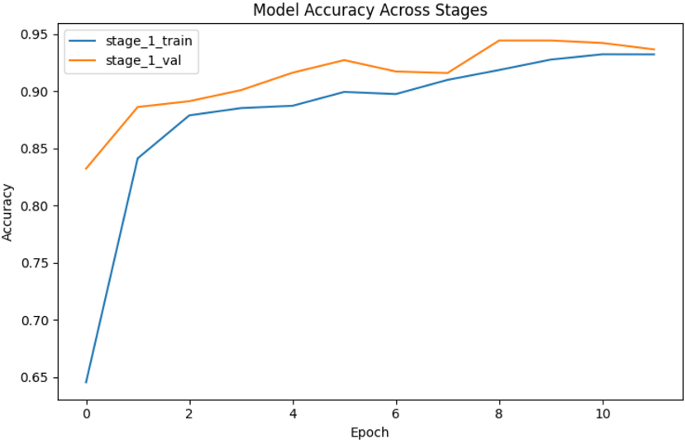
\includegraphics[width=0.5\textwidth]{images/final_accuracy.png}
            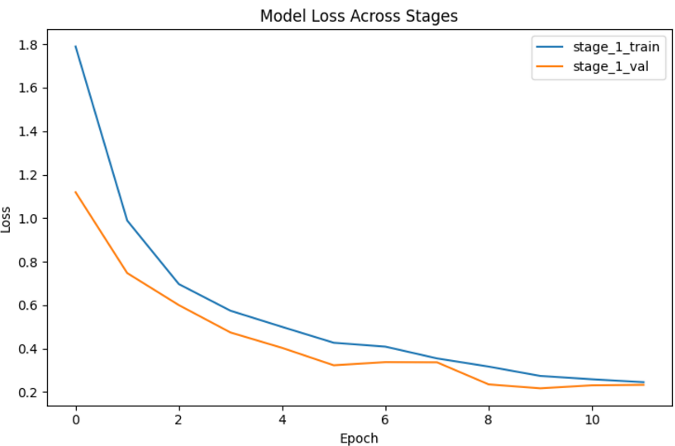
\includegraphics[width=0.5\textwidth]
            {images/final_loss.png}
        \end{figure}
        
        The submission of this final model made us able to achieve a final local accuracy of \textbf{96\%} and an online one of \textbf{92\%}
        
        \section{Contributions}
        Each team member contributed equally, with Bettiati working on environment setup and model training, Bianchi on model building, dataset cleaning and augmentation, and Ostidich on data augmentation and hyperparameter tuning.

        \bibliographystyle{abbrv}
        \bibliography{reports/references}
        
        
    \end{multicols}
\end{document}
        